\documentclass[12pt]{article}
\usepackage{amssymb,amsmath,graphicx,mathtools}
\usepackage{listings}
\usepackage[margin=0.75in]{geometry}
\parindent 16 pt
\usepackage{fancyhdr}
\pagestyle{fancy}
\fancyhead[R]{Swupnil Sahai}
\fancyhead[C]{04/05/16}
\fancyhead[L]{Kernel Model}
\DeclarePairedDelimiter\ceil{\lceil}{\rceil}
\DeclarePairedDelimiter\floor{\lfloor}{\rfloor}

\lstset{
    language=R,
    basicstyle=\scriptsize\ttfamily,
    stepnumber=1,
    numbersep=5pt,
    showspaces=false,
    showstringspaces=false,
    showtabs=false,
    frame=single,
    tabsize=2,
    captionpos=b,
    breaklines=true,
    breakatwhitespace=false,
    escapeinside={},
    keywordstyle={},
    morekeywords={}
    }

\begin{document}

% CUSTOM SHORTCUTS

\def\ci{\perp\!\!\!\perp}
\def\ex{\mathbb{E}}
\def\prob{\mathbb{P}}
\def\ind{\mathbb{I}}
\def\grad{\triangledown}
\def\bigo{\mathcal{O}}

%MODEL FORUMLATION
\subsection*{Motivation}
The previous model using a mixing matrix had bias/variance and identifiability issues because the parameters lacked constraints (other than the rows summing to 1). In an effort to fix this issue, we've now built a model with more structure and far fewer parameters.

\subsection*{Formulation}
We are still using a negative binomial formulation but the expression for the mean has been modified to express mixing using a Gaussian kernel:

$$ y_{ik} \sim \text{NegBin}(\omega_k \mu_{ik}, \omega_k)
\hspace{20 pt} E(y_{ik}) = \mu_{ik} 
\hspace{20 pt} Var(y_{ik}) = \mu_{ik} + \frac{\mu_{ik}}{\omega_k}$$

\noindent  Now let $a_i \in (-\infty,\infty)$ and $g_i \in \{M,F\}$ denote the age and gender of ego $i$, respectively, while we let $g_k$ denote the gender of alter name $k$. Then we can derive the mean expression as follows:

$$ \mu_{ik} = N_i p(k, g_k | a_i, g_i)
= N_i \int_s p(k, s, g_k | a_i, g_i) ds
= N_i \int_s p(k | s, g_k, a_i, g_i) p(s, g_k | a_i, g_i) ds $$
$$ = N_i \int_s p(k | s, g_k) p(s | g_k, a_i, g_i) p(g_k | a_i, g_i) ds
= N_i \int_s p(k | s, g_k) p(s | g_k, a_i, g_i) p(g_k | g_i) ds $$
$$ = N_i p_{g_ig_k} \int_s p(k | s, g_k) \mathcal{K}_{g_ig_k}(a_i, s) ds$$

\noindent where the kernel is parametrized as:

$$ \mathcal{K}_{g_ig_k}(a_i, a_j) = \frac{1}{\sqrt{2\pi\lambda_{g_ig_k}}} e^{-\frac{(a_i-a_j)^2}{2\lambda_{g_ig_k}}} $$

%SIMPLIFICATION%
\subsection*{Simplification Options}
1. If we assume $p(k | s, g_k) \sim \mathcal{N}(\mu_{k}, \sigma_{k})$, we can simplify the integral in the expression of $\mu_{ik}$ using the product of unconstrained normals:
$$ \int \mathcal{K}_{g_ig_k}(a_i, s) p(k | s, g_k) ds
=  \int_{-\infty}^{\infty} \frac{1}{\sqrt{2\pi\lambda_{g_ig_k}}} e^{-\frac{(a_i-s)^2}{2\lambda_{g_ig_k}}} \frac{1}{\sqrt{2\pi}\sigma_{k}} e^{-\frac{(s-\mu_k)^2}{2\sigma_{k}^2}}ds 
= \frac{ e^{-\frac{(a_i-\mu_k)^2}{2(\lambda_{g_ig_k}+\sigma_{k}^2)}} }{\sqrt{2\pi(\lambda_{g_ig_k} + \sigma_{k}^2)}} $$

\noindent We can then reformulate the expectation as such:
$$\mu_{ik} =
\frac{N_i p_{g_ig_k}}{\sqrt{2\pi(\lambda_{g_ig_k} + \sigma_{k}^2)}} e^{-\frac{(a_i-\mu_{k})^2}{2(\lambda_{g_ig_k}+\sigma_{k}^2)}} 
$$

\noindent 2. An alternative simplification is to refactorize $p(k | s, g_k) = \frac{p(s | k, g_k) p(k, g_k)}{p(s, g_k)} = \frac{p(s | k, g_k) p(k | g_k)}{p(s | g_k)}$ and then assume that $p(s | k, g_k) \sim \mathcal{N}(\mu_{k}, \sigma_{k})$ and $p(s | g_k) \sim \mathcal{N}(\mu_{g_k}, \sigma_{g_k})$.

%SIMPLIFICATION VALIDITY%
\pagebreak
\subsection*{Normality Validity}
\noindent To assess the validity of option 1, we present the empirical distributions of $p(k | s, g_k)$:

\begin{center}
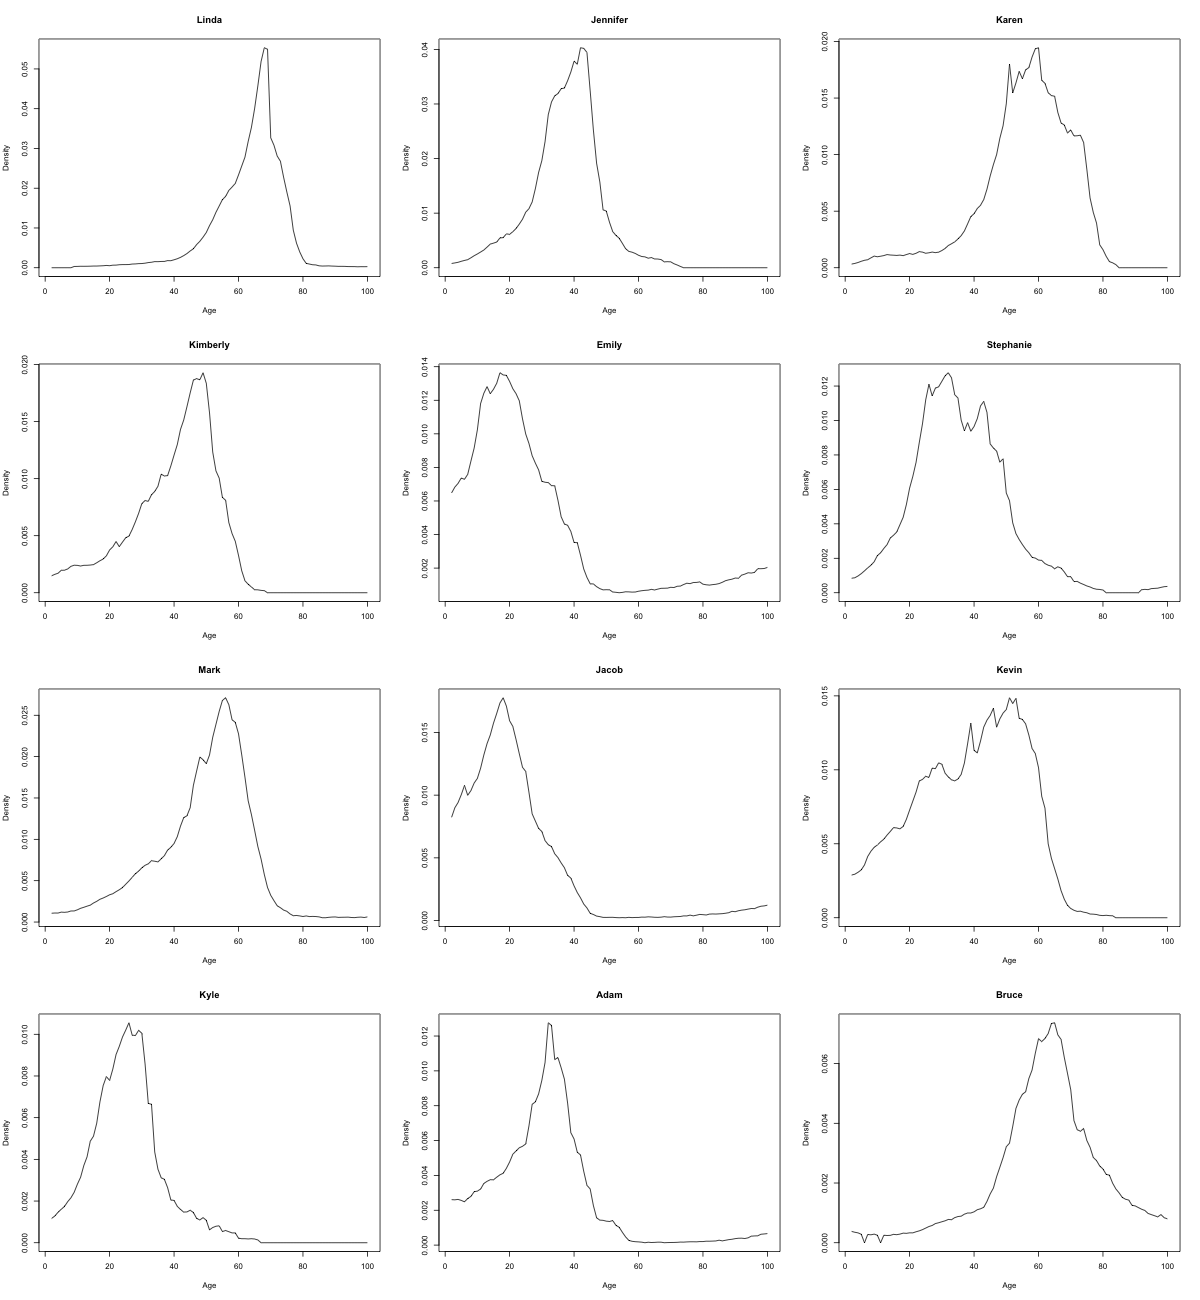
\includegraphics[scale = 0.4]{Option1_Histograms.png}
\end{center}

\pagebreak
\noindent To assess the validity of option 2, we present the empirical distributions of $p(s | k, g_k)$ and $p(s | g_k)$:

\begin{center}
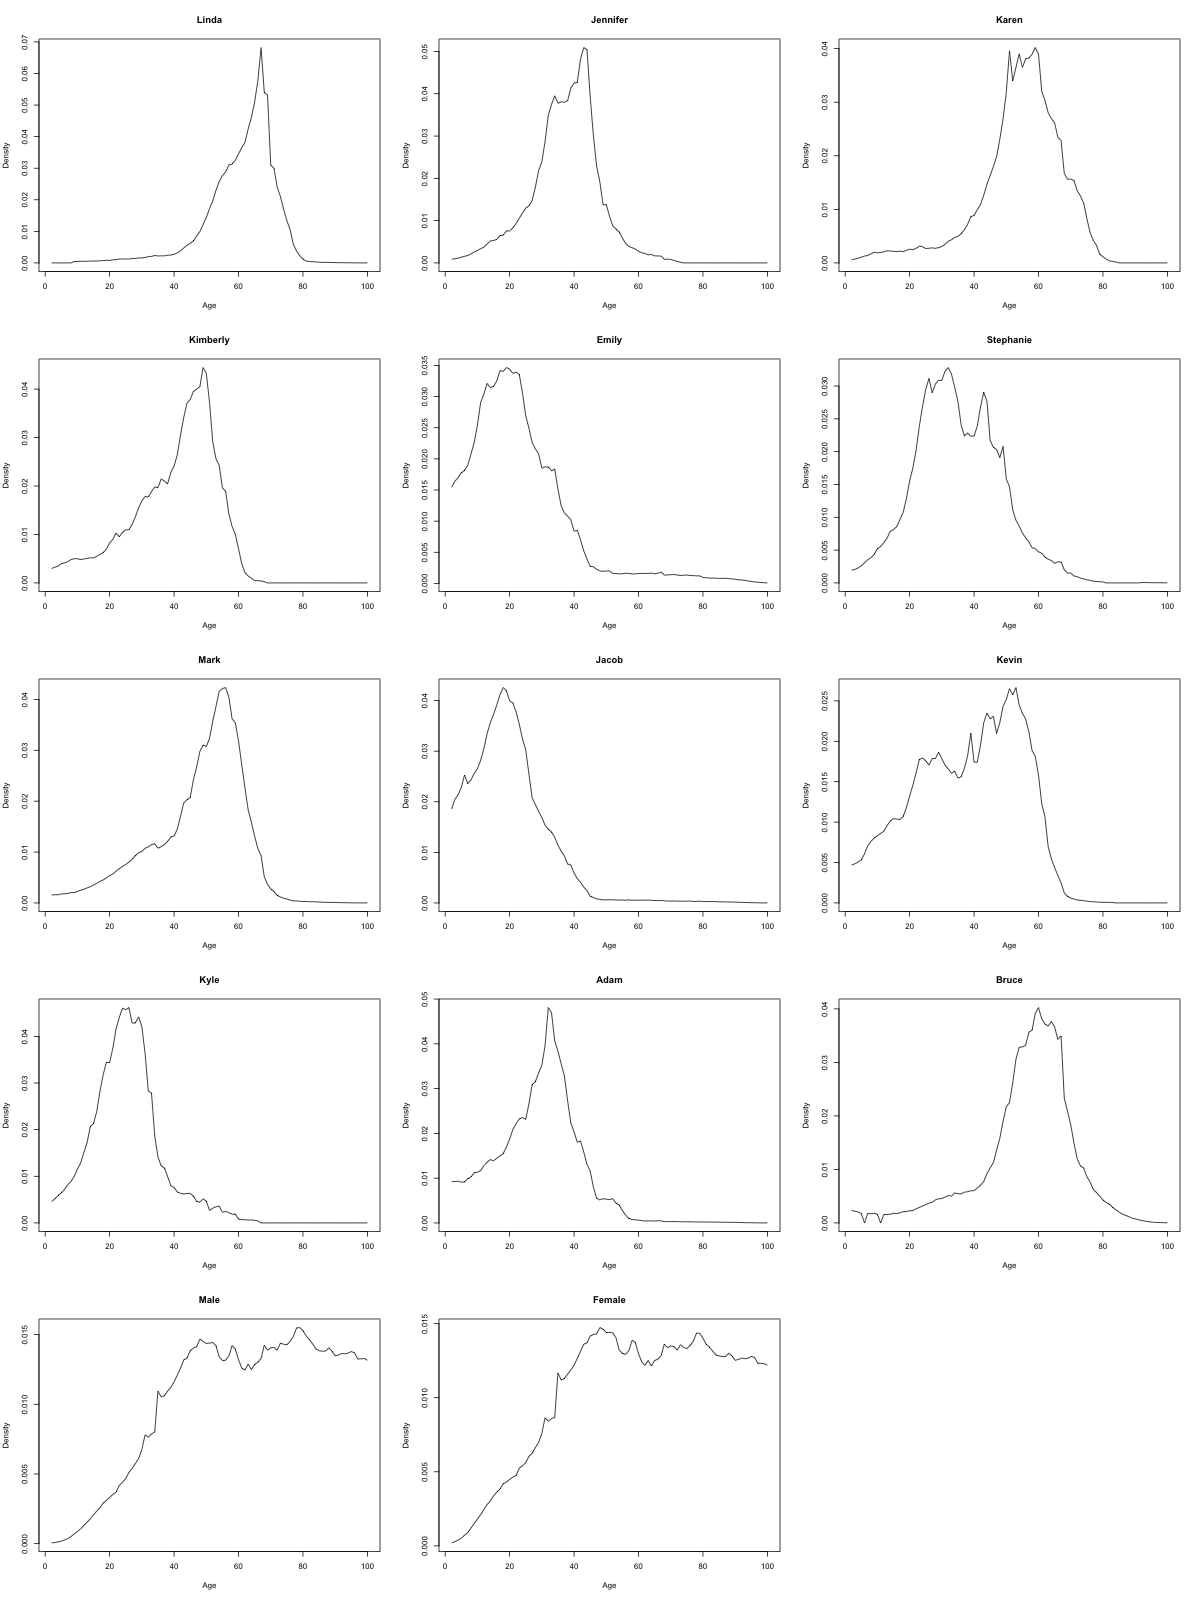
\includegraphics[scale = 0.4]{Option2_Histograms.png}
\end{center}

\end{document}